%!TEX root = ../dissertation.tex
\chapter{Aperture effects in Stellar Mass Estimates}

\label{ch:acm}
\newpage

\section{Introduction}

In this chapter we investigate methods of constraining the star formation histories and stellar masses of galaxies where galaxy spectra are available. In particular, we look at the largest galaxy catalog of estimated stellar masses, star formation rates and gas metallicities, the MPA-JHU catalog \citep{brinchmann_physical_2004, kauffmann_stellar_2003, tremonti_origin_2004}, obtained from spectra from the Sloan Digital Sky Survey (SDSS) Legacy Survey. The MPA-JHU catalog has, over the last decade and a half, been one of the most influential and widely-used catalogs in the fields of galaxy formation and evolution; the original catalog paper of \citet{kauffmann_stellar_2003} has been cited over a thousand times. Here we test a fundamental assumption of the catalog, which is that spectroscopic measurements of the central region of the galaxy yield sufficient information to constrain star formation histories and stellar masses for the galaxy as a whole.\\

The importance of galaxy star formation histories has been discussed in Sections \ref{questions} and  \ref{sec: results}. Crucial to analyzing these histories are accurate inferences of star formation rates and stellar masses from observed data. In particular, the stellar mass function, which is used to calibrate the parameters in simulations that seek to reproduce the star formation histories of galaxy populations, relies on accurate observational calibrations of stellar mass. In this spirit, I examine one of the most widely used stellar mass estimation methods; this method from \citet{kauffmann_stellar_2003} involves two spectral indicators and uses an aperture correction to account for the limited spatial resolution coverage of SDSS spectra. I investigate the robustness of this method using spatially resolved spectra from the Mapping Nearby Galaxies at Apache Point Observatory survey (MaNGA; \citealt{bundy_overview_2014}).\\

\subsection{The SDSS spectra}
\label{sdss spectra}

As introduced in Section \ref{sec: surveys}, SDSS has been conducting a coordinated imaging and spectroscopic survey since 2000 and is currently in its fourth phase of operation. The first two phases of the survey, SDSS and its extension SDSS-II, ran from 2000--2008 and took spectroscopy over approximately 8,000 square degrees of mostly the northern galactic sky 
ran between 2000-2008. It served as the primary database for the MPA-JHU catalog (\citealt{brinchmann_physical_2004, kauffmann_stellar_2003, tremonti_origin_2004}), whose final results were published in SDSS's Data Release 8 (DR8), 
which contains observed spectra of a little over 900,000 galaxies \citep{aihara11a}.\\

The imaging and spectroscopic data were observed using a 2.5 m telescope at the Apache Point Observatory (APO) in Sunspot, New Mexico. The imaging data was obtained by using a wide-field mosaic CCD camera and the spectroscopic data, using twin multi-object fiber spectrographs  \citep{smee_multi-object_2013}, all of which are mounted at the Cassegrain focus of the telescope. The imaging survey, which is carried out in drift-scanning mode using a 5 $\times$ 6 array of 2048 $\times$ 2048 pixel detectors, obtains photometry in the \emph{u, g, r, i} and \emph{z} bands. This broadband photometric data, after reduction and calibration, serves as the pool of data from which spectroscopic target selection is then done. The spectroscopic fiber plug-plates are aluminum plates which have holes drilled into them at positions decided upon by the target selection and the optical fibers are plugged into into these holes. They have a circular field-of-view of radius 1.49 degrees and during SDSS-I and -II were outfitted with 640 fibers, allowing for simultaneous observation of 640 spectra (mostly galaxy spectra and some which are reserved for standard and blank sky observations for calibration) in a 3 degree diameter field of view over the course of a single exposure.\\

The fiber diameter of the optical fibers was chosen with a view to maximize the signal-to-noise (S/N) ratio for an extended source, keeping in mind the sky conditions at APO. The optimal choice that was decided upon corresponds to a fiber diameter of 180 $\mu$m or 3''. The rest-frame wavelength range of the spectra at the median redshift is from 3500 \AA\ to 8500 \AA\ with a spectral resolution:\\ $$R = \frac{\Delta \lambda}{\lambda} \approx 2000.$$ The spectra are calibrated using observations of F stars in each 3 degree field.\\

SDSS imaging data and spectra have played a significant role in many discoveries in astronomy and cosmology over the last decade and a half. In addition to fundamental measurements of cosmological parameters and the study of distant quasars and stars in our own galaxy, the Main Sample of galaxies in SDSS-I and -II (\citet{strauss02a}) has informed much of the new understanding of galaxy properties that we have today. This 
new understanding has included the quantification of the 
bimodal nature of galaxy properties {\bf cites}, the relationship
between galaxy properties and environment {\bf cites}, and
how galaxy properties relate to the masses and other properties
of their host dark matter halos {\bf cites}. Key to many 
of these  works has been the use of new ways to estimate
star formation histories, stellar masses, and chemistry of 
stars in galaxies, including those found in the MPA-JHU 
catalog.
I discuss the catalog and the methods used to estimate these quantities in the following sections.\\

\subsection{The MPA-JHU Catalog}

The MPA-JHU catalog is the result of a collaborative effort between a group of researchers at the Max Planck Institute for Astrophysics and the John Hopkins University and was first constructed for the first SDSS Data Release (DR1) of spectroscopic observations. The original dataset they used was 120,808 galaxies drawn from the SDSS DR1 for which the following properties were estimated: stellar masses and mass-to-light ratios, effective stellar attenuation by dust, indicators of recent major starbursts, current total and specific star-formation rates, gas-phase metallicities, AGN classifications based on the standard emission line ratio diagnostic diagrams and AGN luminosities. The methods of estimation of these properties can be found in \citet{kauffmann_stellar_2003} for the stellar masses, \citet{brinchmann_physical_2004} for the star formation rates and \citet{tremonti_origin_2004} for the gas phase metallicities.\\

The MPA-JHU catalog measurements are ubiquitous in galaxy evolution literature with many important results relying on the inferred SFR's, masses and metallicities from the catalog. A few examples of scientific results from which the significance of the catalog can be evinced would be: understanding the host galaxies of AGN's by Kewley \citep{kewley2006}, the star formation-density relation and its reversal in distant universe by \citet{elbaz2007}, constraining the mass-metallicity relationship for star-forming galaxies \citep{kewley2008}, the mass dependence of radio-loud AGN's \citep{best05a}, insights into quenching mechanisms \citep{peng_mass_2010} and large scale galactic conformity \citep{kauffmann2013}, mapping the stellar mass function \citep{2009MNRAS.398.2177L, 2015MNRAS.454.4027D}, and many others.\\

The MPA-JHU catalog uses SDSS spectra to constrain the stellar masses and star formation histories in the catalog by looking at two key spectral indicators of starbursts and age of a galaxy: the Balmer ${\rm H}\delta_{\rm A}$ absorption line index and the ${\rm D}_{\rm n}4000$ break index.   Because they are both measurements defined over a narrow range of wavelengths in the blue, that are similar to each other, and are independent of the absolute flux, they are designed to be insensitive to dust extinction within the galaxy. The indices are discussed in detail in Sections \ref{d4000} and \ref{hdelta}. Using the distribution of the observed galaxies in the ${\rm H}\delta_{\rm A}-{\rm D}_{\rm n}4000$ plane and by employing Stellar Population Synthesis (SPS) models by \citet{bruzual_stellar_2003-1} to model the evolution of galaxies in this plane, they are able to derive maximum likelihood estimates of the stellar mass of a galaxy \citep{kauffmann_stellar_2003}, the attenuation of optical light by dust and the fraction of stars in a galaxy formed in recent bursts.\\

The spectra are only of the center of the galaxy so do not on their own constrain the total stellar mass. What is actually inferred from each spectrum at a given point ${\rm H}\delta_{\rm A}-{\rm D}_{\rm n}4000$ phase space is the mass-to-light ratio in the $z$-band for models that are at that same point. Now, as we have just seen in Section \ref{sdss spectra}, due to the nature of fiber spectroscopy, the angular area of coverage of a galaxy observed is limited to 3$''$, which could correspond to different actual physical sizes depending on the redshift of the galaxy. Thus, \citet{kauffmann_stellar_2003} (and in a similar way for SFRs, \citealt{brinchmann_physical_2004}) prescribe a method of aperture correction that relies on the assumption that the mass-to-light ($M/L$) ratio of the central part of a galaxy is representative of the entire galaxy. Thus the fiber M/L ratios are obtained in the \emph{z}-band are multiplied by the luminosity of the galaxy in the \emph{z}-band, that can be obtained from SDSS broadband photometry accounting for 
the full flex of the galaxy and thus presumably the 
total stellar mass of the galaxy. The methodology and the motivations behind it are discussed in further detail in Section \ref{kauffmann method}.\\

It follows from the above that the MPA-JHU catalog stellar 
masses would be systematically affected whenever the 
central $M/L$ ratios were not representative of the 
entire galaxy. For example, the bulge and disk components
of luminous spiral galaxies have systematically different
star formation histories and thus mass-to-light ratios; 
since the bulge dominates the inner part of the galaxy,
it can potentially dominate the fiber spectrum and yield
a $M/L$ unrepresentative of the galaxy as a whole.
To quantify exactly how this systematic affects
MPA-JHU masses  spatially resolved spectra for galaxies
is necessary.
Integral Field Unit (IFU) based surveys provide us the 
necessary data to be able to do that. In the following
section, I review briefly  the field of integral field spectroscopy and describe in more detail the MaNGA survey
\citep{bundy_overview_2014}.

\subsection{Integral Field Spectroscopy and MaNGA}

Integral Field Spectroscopy in astronomy is motivated
by the need to study the variation of spectra across
extended objects, in order to determine its internal
structure and dynamics.
An Integral Field Unit (IFU) enables the observation 
of multiple regions of the extended object simultaneously 
to obtain these spatially resolved spectra. There are many 
ways of doing this, including and not limited to image 
slicers, lenslet arrays, and multi-fiber IFUs. As we 
have seen in Section \ref{sdss spectra}, while 
spectroscopic surveys have created huge breakthroughs 
in galaxy evolution and cosmology alike, their restricted 
spatial coverage has resulted in the need for more or 
less uncertain aperture corrections to measure properties
of the galaxy as a whole, and in the inability to 
make reliable inferences about galaxies' internal structure.

Some noteworthy IFU-based surveys include the 
Sydney-Australian-Astronomical-Observatory Multi-object Integral-Field Spectrograph (SAMI; \citealt{bryant_sami_2015}), the 
Multi Unit Spectroscopic Explorer (MUST; \citealt{bacon_muse_2015}), and the Calar Alto Legacy 
Integral Field Area Survey (CALIFA; \citealt{sanchez_califa_2012}). 
Over the last decade these and other surveys have
contributed greatly to our understanding of the internal 
lives of galaxies. 
For the purposes of this project, 
the survey that bests suits our purposes is 
MaNGA (Mapping Nearby Galaxies at Apache Point \citep{bundy_overview_2014}). MaNGA is the largest 
IFU-based survey undertaken so far in terms of 
numbers of galaxies, planning to obtain spatially 
resolved spectra of about 10,000 galaxies by 2020. 
This size and the homogeneous selection of 
galaxies is one important consideration 
(Section \ref{mangadrp}). Another important 
consideration is that it uses the BOSS spectrograph,
which is very similar to the original SDSS spectrograph,
and the data is calibrated and processed using very
similar methods to SDSS-I and -II data.
These properties make it a natural sample to use
to test systematics in the methods applied to 
the MPA-JHU catalog.

MaNGA uses 17 multiple fiber IFUs simultaneously
\citep{drory_manga_2015}.
In the same way that single fibers are plugged into 
plates (Section \ref{sdss spectra}), the multiple 
fiber bundles are plugged at the appropriate 
locations on plug-plates to be observed at the 
focal plane of the 2.5m telescope at Apache Point. 
The fibers are 2.0$''$ in size and the bundles 
themselves come in five sizes and contain 19, 
37, 61, 91 or 127 fibers. The bundle assigned to 
each galaxy is determined from the 
angular size of the target galaxy. 

The fibers are arranged in a hexagonal pattern, 
and several observations are taken slightly offset 
from each other (``dithered'') to produce a denser 
hexagonal sampling. During data processing, the 
observations are interpolated onto a rectangular 
grid at each wavelength. 
Each grid point is called a spaxel, which can be 
thought of as a spectrum for every two-dimensional 
pixel. The resulting MaNGA galaxy outputs are 
thus three dimensional ``datacubes" with two 
spatial dimensions and one spectral dimension. 

Each bundle also contains sky fibers to allow for 
very precise sky subtraction by looking at a region of 
the sky that is within a few arcminutes of the target. 
At a given time, MaNGA is able to target 17 galaxies 
(and 12 standard stars) in the 3 degree FOV with much 
wider and continuous wavelength coverage than other
large IFU-based surveys.\\

\section{The $H\delta_{\rm A}-D_{\rm n}4000$ plane}
\label{indices}

In this section, I review the two spectral diagnostic tools used by the MPA-JHU catalog to constrain stellar masses and star formation histories in galaxies, the Balmer $\delta$ absorption line index and the ${\rm D}_{\rm n}4000$ break index in the optical spectrum of a galaxy. Following that I describe the method used by \citet{kauffmann_stellar_2003} to obtain the mass-to-light ratios of galaxies using these indices and finally the aperture correction method used to tranform the fiber masses obtained to the total stellar mass of the galaxy.\\

\subsection{The $D_{\rm n}4000$ break in Galaxy Spectra}
\label{d4000}

Spectral discontinuities in stars can be 
produced by the accumulation of a large number 
of spectral lines in a narrow region. 
In certain cases this can lead to a relatively 
sharp discontinuity, or ``break,'' in  the 
spectrum of the star.  
A prominent break in galaxy spectra occurs in the
optical at 4000 
\AA \citep{bruzual1981, bruzual_a._spectral_1983}, 
which exists in the spectra of K stars and thus 
appears in stellar populations older than a few
billion years, which are dominated
by K giants. Because it is associated with this 
late stage in the evolution of stellar populations,
the strength of this break is an indicator of the 
mean stellar age over the past few billion years.

The specific metallic absorption lines causing the break 
include a variety of elements in varying states of 
ionization, including including the CaII doublet, H 
and K (3969 \AA and 3934 \AA) and higher order 
Balmer lines such as H$\epsilon, \lambda$, etc. 
\citep{hamilton1985}. As the break does tend to be pronounced in intermediately old stellar populations which tend to be metal rich, it does depend on stellar metallicity, exhibiting some of the same age-metallicity degeneracy that afflicts most spectroscopic indicators.\\ 

%The so-called 4000 \AA\ break is produced by the absorption of metallic lines of a variety of elements in various states of ionization,  The opacity suddenly increases for photons bluer than this wavelength, which produces an intensity drop. It is enhanced in old stellar populations, which tend to be metal rich, but it is also present in younger galaxies.

%The most obvious discontinuity in the spectrum of a galaxy is often the $D_{n}4000$ break \citep{1999ApJ...527...54B}, which is a consequence of the absorption into electronic excited states by neutral and partially ionized metals whose lines happen to overlap in the region just blueward of 4000 \AA.  Older stellar populations have spectra dominated by relatively cool giant stars, and under these conditions the partially ionized metal lines are strong. Younger stellar populations have spectra dominated by hot stars, for which these lines are weaker. 

This break was defined in by \citet{bruzual_a._spectral_1983-2} as the ratio of the average flux density $F_{\rm \nu}$ in two bands that span \textasciitilde200 \AA on either side of 4000 \AA. \citet{1999ApJ...527...54B} defined a narrow band definition for the same where the bands that are now 100 \AA wide with 3850 \AA - 3950 \AA as the ``blue continuum" and 4000 \AA - 4100 \AA as the ``red continuum". The bandpass used in \citet{kauffmann_stellar_2003} (\ref{fig:early_late_type}) is the same as the one introduced by \citet{1999ApJ...527...54B} and their motivation for doing so is that the narrow definition is more insensitive to reddening effects. I reproduce these measurements using the same narrow band definition.\\

\begin{figure}
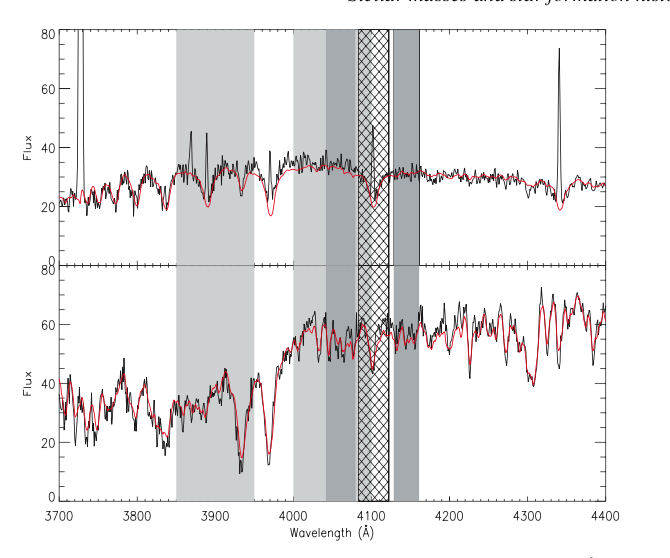
\includegraphics[width=\textwidth]{figures/spectra_placeholder.png}
\caption[PLACEHOLDER FIG; TBD: A figure showing D4000 and Hdelta breaks in spectra for early/late-type galaxies as well as the bimodality in D4000
]{ PLACEHOLDER FIG; TBD: A figure showing D4000 and Hdelta breaks in spectra for early/late-type galaxies as well as the bimodality in D4000
\label{fig:early_late_type}}
\end{figure}


\begin{figure}
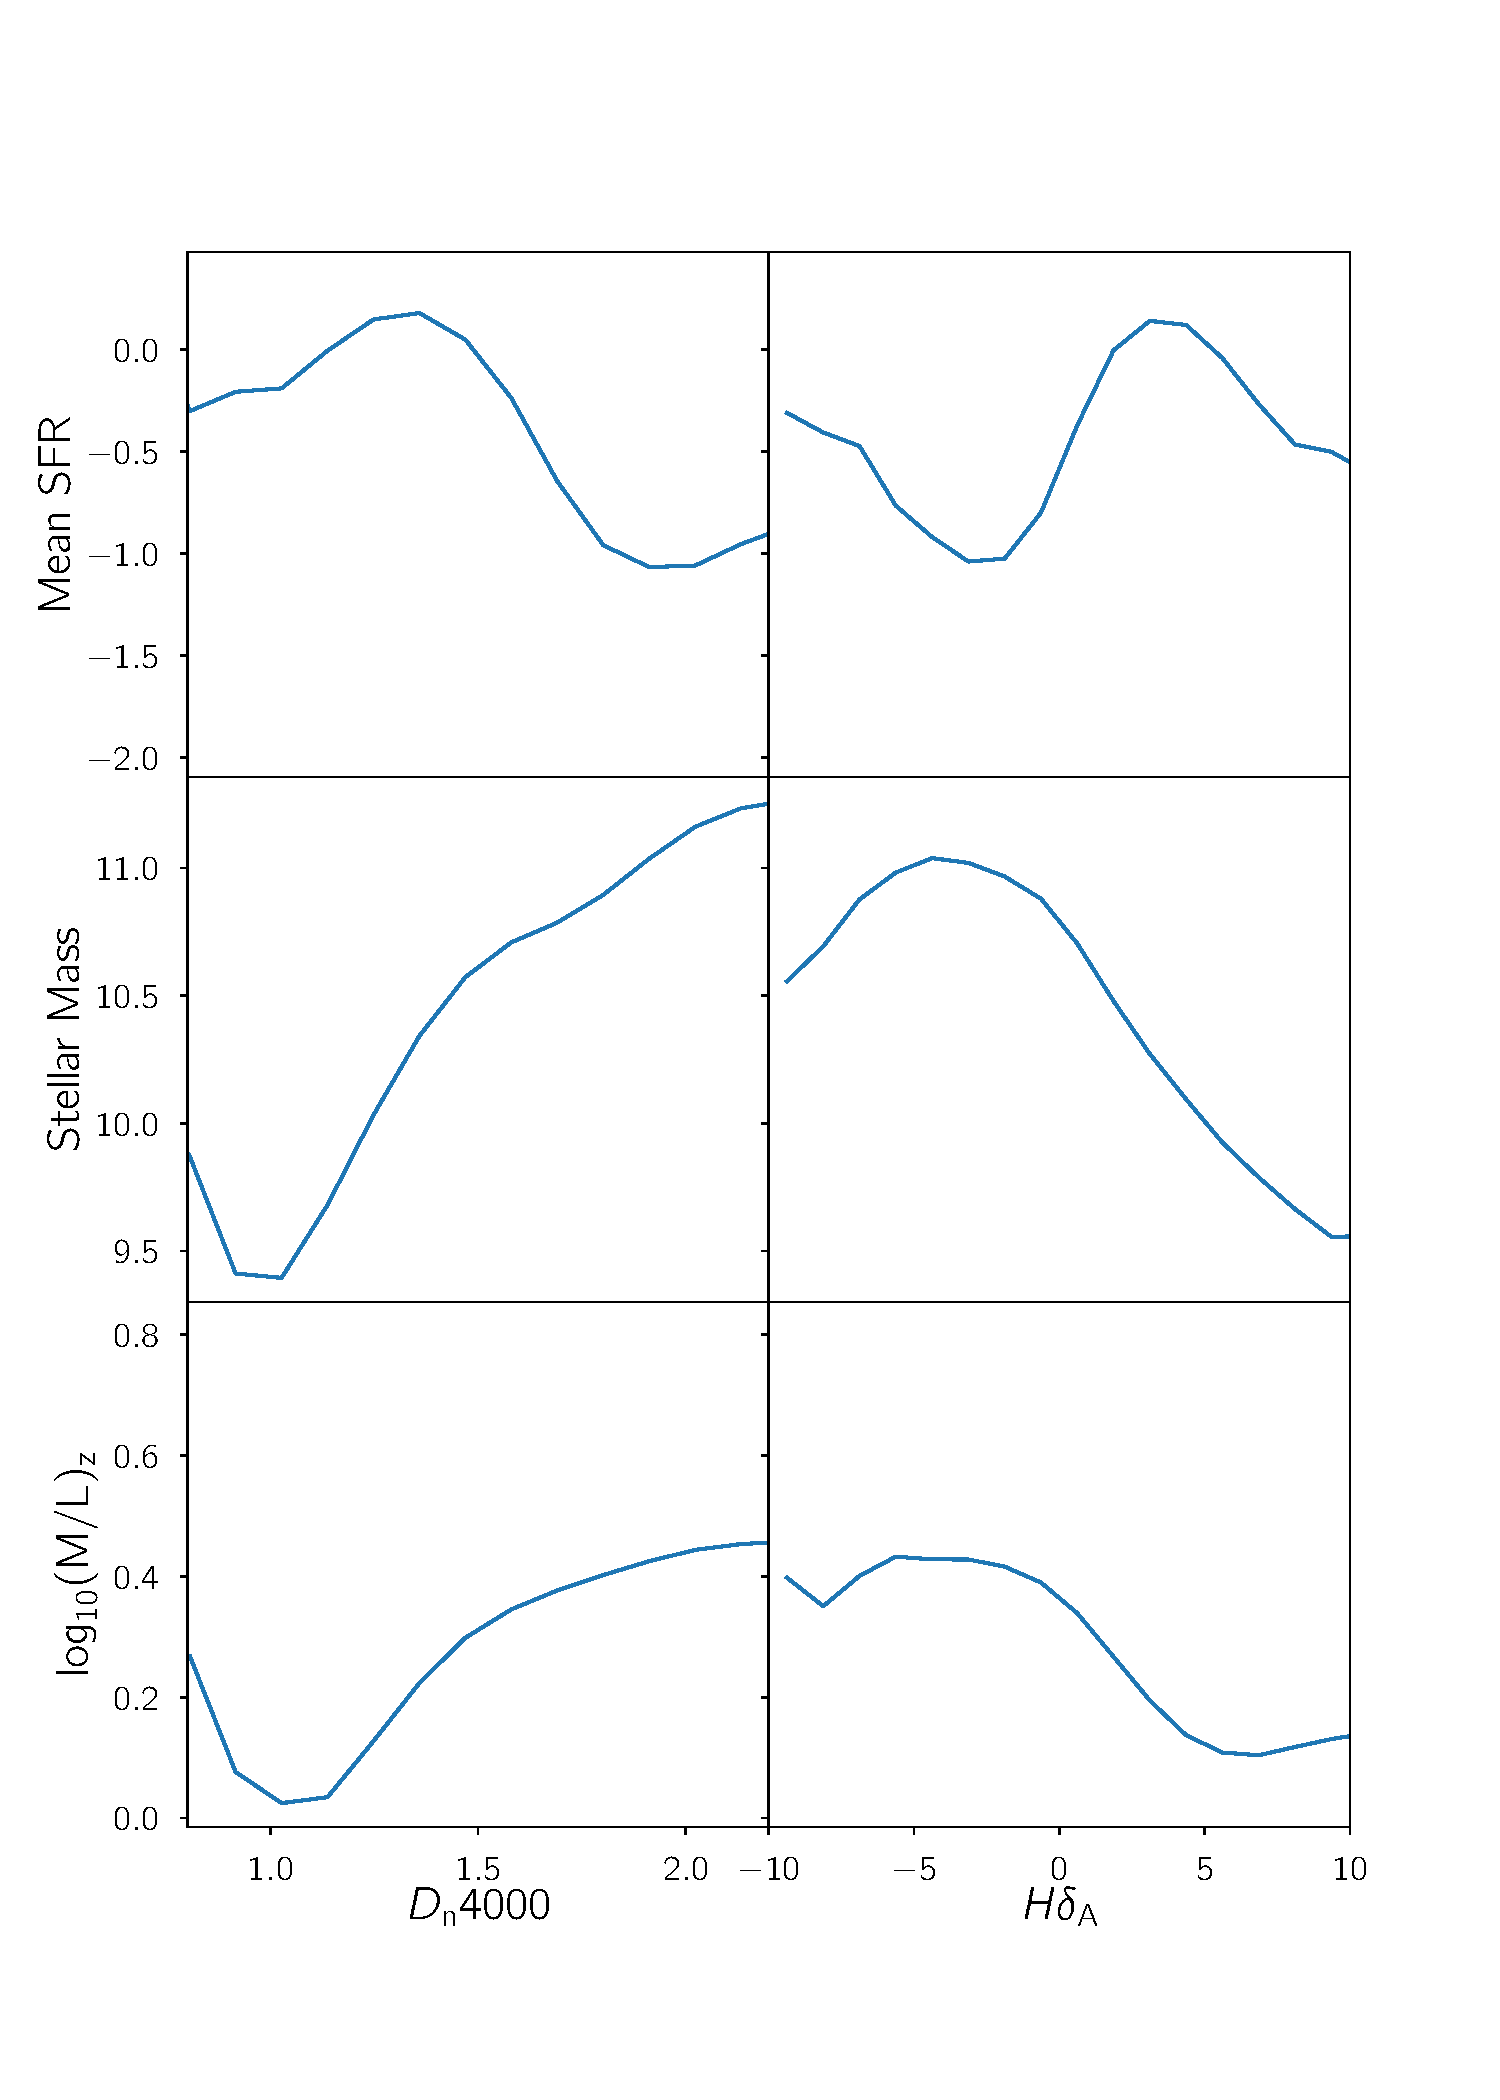
\includegraphics[width=\textwidth]{figures/mass_age_sfr_dist.pdf}
\caption[SFR's, stellar masses, ages and Mass-to-light ratios as a function of H$\delta_{\rm A}$ and ${\rm D}_{\rm n}4000$ for the DR8 SDSS galaxies ]
{Stellar masses, ages and Mass-to-light ratios as a function of H$\delta_{\rm A}$ and ${\rm D}_{\rm n}4000$ for the DR8 SDSS galaxies: \emph{Age needs to be included}
\label{fig:sfr_mass}}
\end{figure}


\subsection{The Balmer H$\delta$ Absorption Line}
\label{hdelta}

As we have seen in Section \ref{sed}, the spectral features of galaxies contain a wealth of information about their star formation properties. In particular the Balmer lines in the optical are very useful in understanding the ionized hydrogen content in the stellar populations in the galaxies and can thus provide valuable insight into star formation properties. The Balmer emission lines are the result of re-emission of light from hot, young stars by the ISM or HII regions in galaxies as we have seen in Section \ref{sfrs}. The absorption lines such as the H$\beta$, H$\gamma$ and H$\delta$ absorption lines, however, are characteristic of stellar spectra (predominantly occurring in A-type stars) and are thus tracers of the age and metallicity of stellar populations in galaxies. In particular, a strong H$\delta$ absorption feature is indicative of a starburst having happened 0.5-1.5 Gyrs ago \citep{1983ApJ...270....7D}, assuming that the stellar populations involved are mostly A-type stars.\\

The evolution of the Balmer absorption line profiles in stellar spectra with age points to a tendency for the width of the lines to increase with the age of the stars until about 0.5 Gyr for stellar populations with solar metallicity. Up until ages of about 1 Gyr, the Balmer lines of individual stars are not dependent on metallicity. However the interpretation of stellar age from the integrated light from stellar populations can still be affected by metallicity considerations as lower metallicity stars evolve more slowly in the HR diagram with the strength of the absorption feature peaking at ages older than 1 Gyr. Thus a lower metallicity stellar population at an older age would exhibit a similar H$\delta$ absorption feature as an intermediate-age stellar population with solar (or higher) metallicity.\\

The distinguishing factor, however, in the way the age-metallicity degeneracy affects the Balmer lines as opposed to the metallic absorption features is that the latter is tied more to the presence of the red giant branch stars and the former is more a consequence of the dependence of the main sequence turnoff temperature being a function of metallicity. Thus with the appropriate SPS models, both the mean age and metallicity can be simultaneously obtained. Particularly useful in this endeavor are the Lick indices, obtained by using stellar spectra from the Lick Observatory \citep{1997ApJS..111..377W, worthey_comprehensive_1994}. The Lick indices are a system of 25 line indices, that can successfully disentangle the effects of age and metallicity for a given [$\alpha$/Fe] abundance ratio.\\ 

Measuring an absorption feature involves measuring the flux in a central bandpass relative to two pseudo-continuum bandpasses on either side. A line is drawn between the midpoints of the two flanking pseudo-continuum bandpasses to define the continuum from which an equivalent width is measured by integration. The bandpass definitions we use here, as defined by \citet{worthey_comprehensive_1994} are: an index Bandpass from 4083.50 - 4122.25 \AA with the blue and red bandpasses on either side being 4041.60 - 4079.75 \AA and 4128.50 - 4161 \AA respectively.

\subsection{Constraining SFH's using H$\delta_{\rm A}$ and $D_{\rm n}4000$}
\label{kauffmann method}

The MPA-JHU measurements of stellar masses and ages rely on the results concerning the evolution of the H$\delta_{\rm A}$ and $D_{\rm n}4000$ indices for stellar populations. The evolutionary tracks of these indices with age are mapped by the spectral library, STELIB, incorporated into the SPS models \citep{bruzual_stellar_2003} that are used to fit the SDSS spectral data and the significant observation here is that at a given value of $D_{\rm n}4000$, a stronger H$\delta_{\rm A}$ feature is indicative of recent starbursts. While the evolution of each index with age is not independent of metallicity as we have seen above, together, the locus of galaxies in the H$\delta_{\rm A}$-$D_{\rm n}4000$ plane can provide constraints on the starburst histories of the galaxies. \citet{kauffmann2013} exploit this result to constrain the stellar mass-to-light ratios of galaxies by using a Bayesian inference technique. The prior distribution is a library of models that are generated by Monte Carlo realizations which are representative of both bursty and continuous star formation histories. The library consists of 32000 different star formation histories and their parameter space includes the H$\delta_{\rm A}$ and$D_{\rm n}4000$ indices, the stellar mass-to-light ratios in the z-band, the $g-r$ and $r-i$ colors and the fraction of stellar mass formed in bursts over the past 2 Gyr.\\

This library of models thus enables the construction of a ``model grid" in the H$\delta_{\rm A}$-$D_{\rm n}4000$ plane that maps to various physical properties of the galaxy. For each galaxy in SDSS DR8, the spectra are processed using the SPECTRO2D pipleine and the spectral indices as well as emission line fluxes are calculated using a special purpose code \citep{tremonti_origin_2004} that recovers the best fit model spectrum for each galaxy based on the \citet{bruzual_stellar_2003} SPS models. Thus for each galaxy in the sample, there is an associated value of H$\delta_{\rm A}$ and $D_{\rm n}4000$, along with an error estimate and can now possibly be associated with a model from the library of star formation histories. As the prior on the distribution of the SFH's is akin to the parameter space being Monte Carlo sampled, the likelihood of the distribution of the data given the parameters can be assumed to be Gaussian. The median value of the posterior probability distributions of the parameters for each galaxy derived thus is then used as the ``best" estimate in the catalog. The resulting mass-to-light ratios for the SDSS DR8 galaxies in the H$\delta_{\rm A}$-$D_{\rm n}4000$ plane thus obtained are plotted in Figure \ref{fig:kauff_grid}.\\ 

\begin{figure}
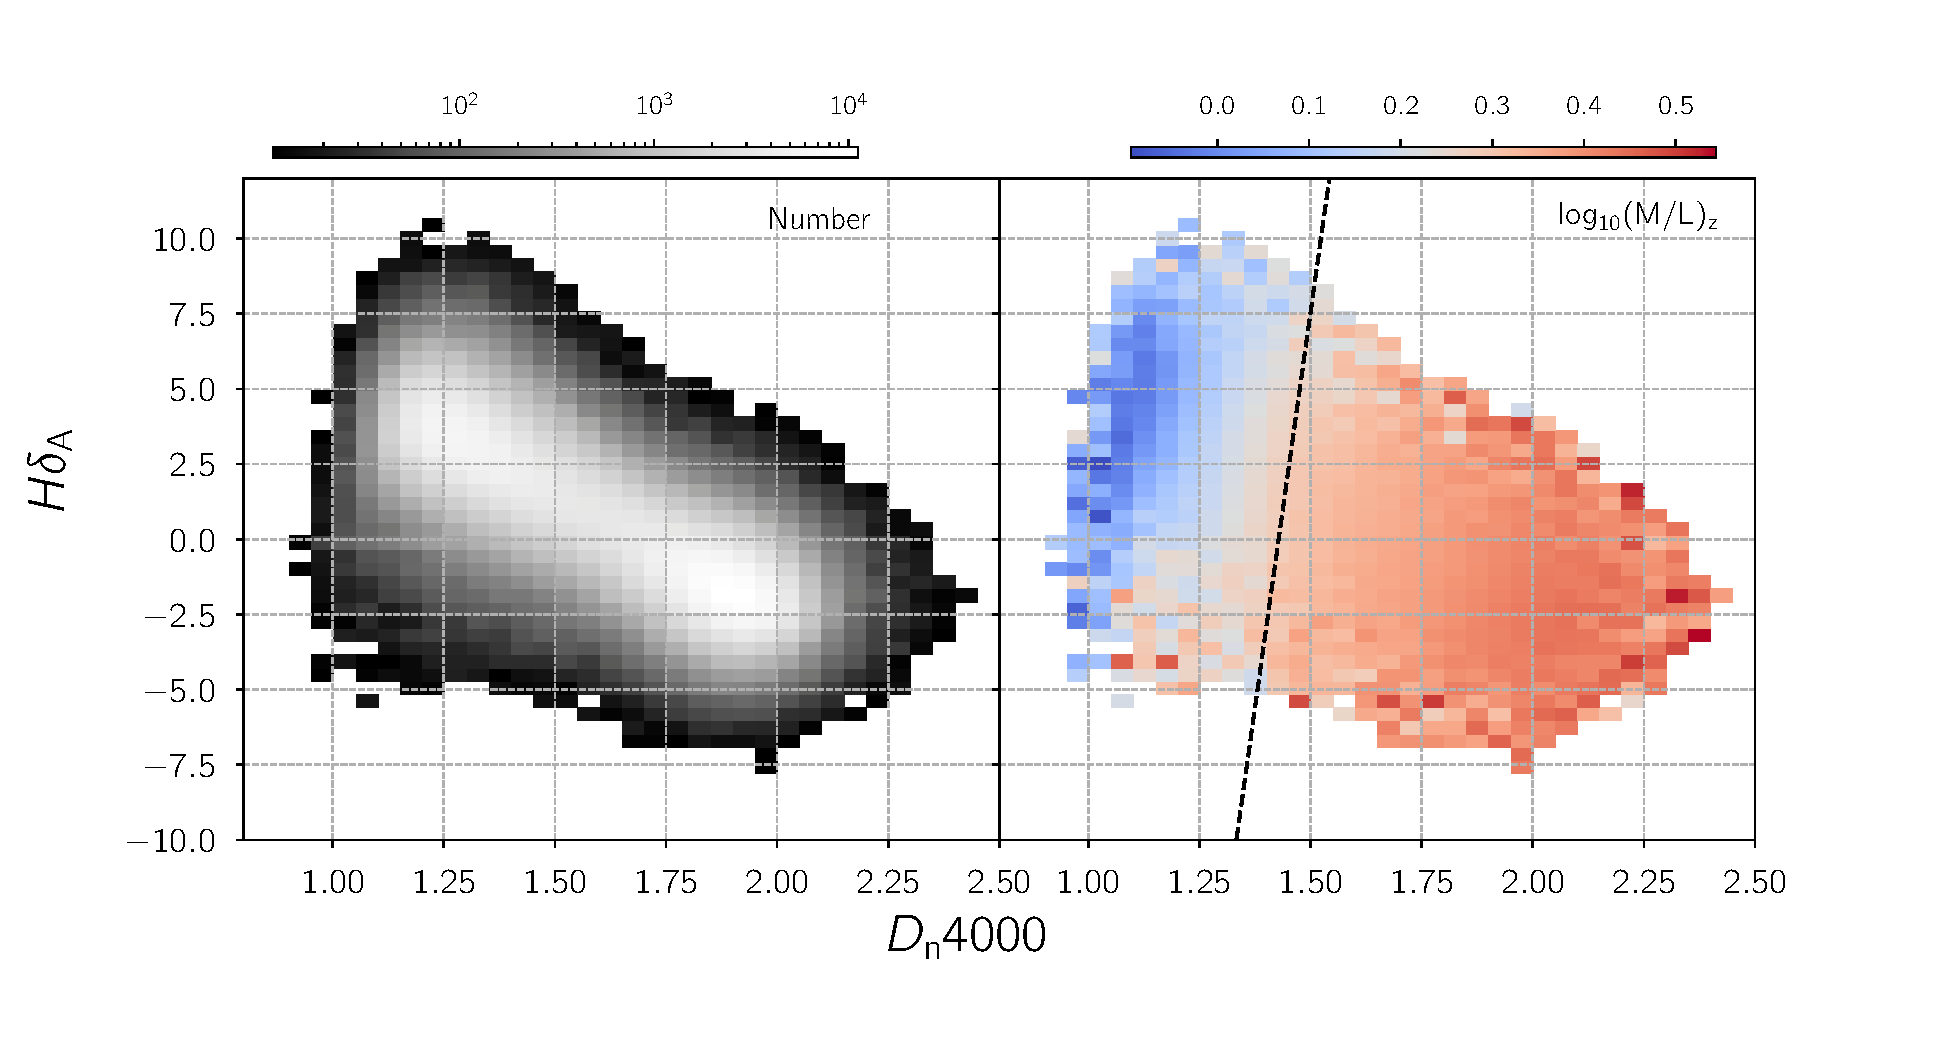
\includegraphics[width=\textwidth]{figures/hd_d4000_mlratio_coarser_binning.pdf}
\caption[The \citet{kauffmann_stellar_2003} grid to infer M/L ratios from the $h\delta_{A}-D_{n}4000$ plane]
{The \citet{kauffmann_stellar_2003} grid to infer M/L ratios from the $h\delta_{A}-D_{n}4000$ plane
\label{fig:kauff_grid}}
\end{figure}

\subsection{The Stellar Mass Aperture Bias in MPA-JHU}
\label{apercorr}

As we have reviewed in Section \ref{sdss spectra}, the SDSS spectra capture starlight within the 3'' aperture diameter with fibers that have been placed as close to the centre of a galaxy as possible and thus there has to be a reasonable way of translating the ``fiber" mass-to-light ratios discussed above to total stellar masses, etc. The MPA-JHU catalog utilizes the broadband photometry data to obtain total stellar masses by multiplying the z-band mass-to-light ratios with the dust-corrected z-band Luminosity of the galaxies, thus extrapolating the fiber mass-to-light ratios and dust attenuation factor to the whole galaxy. Thus it can be expected that the aperture bias in stellar mass would be a strong source of systematic error here, as discussed in \citet{kauffmann2013} (and \citet{brinchmann_physical_2004} for the star formation rates).\\

The most severe scenario for this bias would be in the case of spiral galaxies with star forming discs where the index measurements in the central bulge would not be reflective of the galaxy properties as a whole at all. \citet{kauffmann2013} attempt to address this bias by comparing similar galaxies at different redshifts by using distance as a proxy for the fraction of galaxy that would fall within the aperture to see how significant the shift in the z-band M/L ratios are.\\


\section{Data}

\subsection{MaNGA Target Selection and DRP}
\label{mangadrp}
Primary and Secondary Samples. NSA redshifts/Luminosity cut.


Why Manga is ideal to test the MPA-JHU aperture correction.

\subsection{Our Sample}
The most recent MaNGA product launch, MPL-$8$, which was announced in November $2018$, containing products based on galaxy and stellar library observations from March $2014$ - July $2018$ serves as the source of our sample. It contains $950$ plates - $6779$ data cubes and $20649$ stellar library stars. Out of these, $6468$ are galaxies with measured NSA redshifts. These are representative of all the IFU sizes (list them: 19,37... 127) and span a redshift range upto $z = 0.15$.\\
For each galaxy observation, depending on the IFU bundle size (say $N_{X}$, $N_{Y}$ each describing a position $0.5$" from the previous spaxel), we have ($N_{X}$, $N_{Y}$) spectra which span $4563$ wavelength points. 

\section{Methods}
\label{sec:chap2methods}

\subsection{Variable Aperture Measurements}
For any given datacube, we can determine which spaxels fall within an aperture radius of $R$ arc-seconds as follows. As each spaxel spans a width of 0.5'' in along the ``X" and ``Y" direction, at any point $(x,y)$ in the IFU image, the distance in arc-seconds of the centre of a spaxel from the central spaxel $(x_{c},y_{c})$ in the IFU would be:
$$ d = (r(x,y) - r(x_{c},y_{c})) = \sqrt{(0.5*x)^2 + (0.5*y)^2} $$
Thus, for every spaxel in the IFU, where $d<=R$, that part of the galaxy would fall within the aperture and hence, we would include that spaxel in the measurement of whichever spectral index. Using this, for instance, we can simulate the SDSS fiber measurement, i.e.,  what the $1.5$" aperture radius used in SDSS would see versus the total galaxy or what we call a ``full aperture" measurement.

%\begin{figure}
%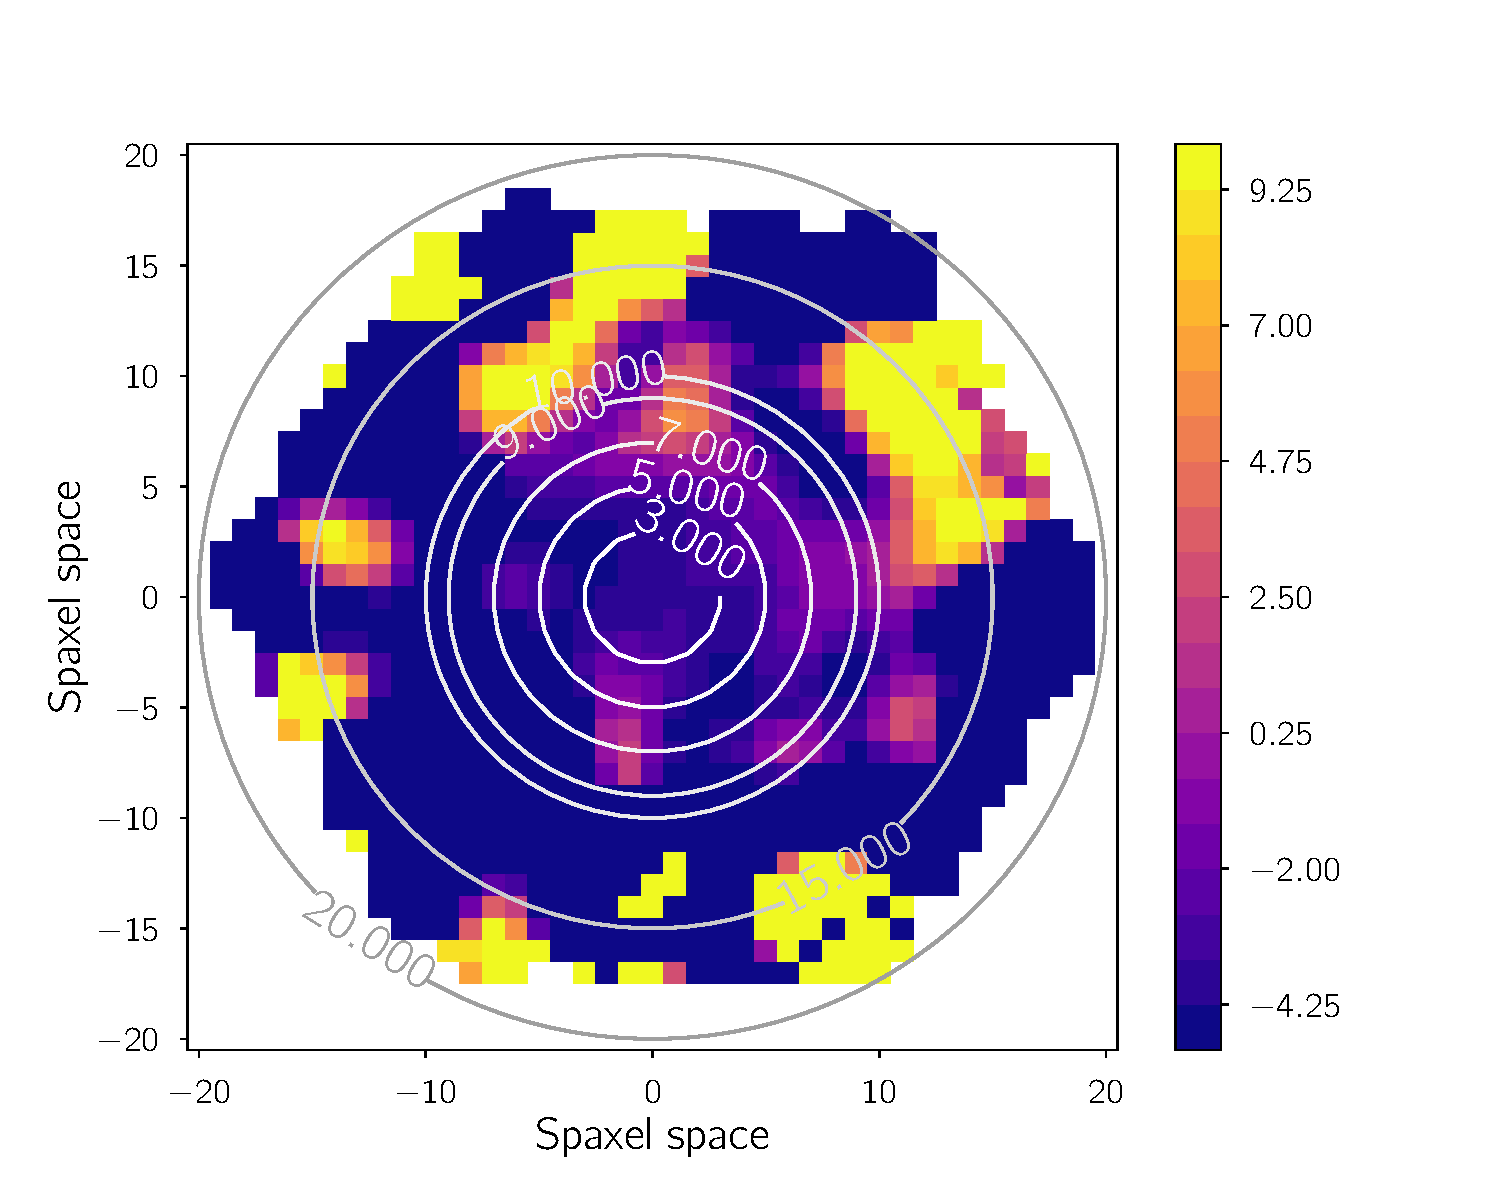
\includegraphics[width=\textwidth]{figures/gal_aperture.pdf}
%\caption[Placeholder figure: TBD. Sample MaNGA galaxy view in the spaxel space with the $H{\delta_{\rm A}}$ distribution plotted as a function of position and the contours marking the aperture diameters at different angular distances in arcseconds]
%{Placeholder figure: TBD. Sample MaNGA galaxy view in the spaxel space with the $H_{\delta_{\rm A}}$ distributions plotted as a function of position and the contours marking the aperture diameters at different angular distances in arcseconds
%\label{fig:sample_manga}}
%\end{figure}

One can alternately pose this question in terms of redshift. For all galaxies whose redshift $z_{\rm obs}$ is less than the redshift we are interested in, $z_{\rm cutoff}$, we can ask the question: if we shift the said galaxy to the said cutoff point, where would its location on the $H\delta_{\rm A}$ - $D_{\rm n}4000$ plane be? How offset is this from the ``full aperture" measurements?\\

Transverse angular distance varies with redshift as follows:
$$D_{\rm A}(z) = \frac{D_{\rm M}(z)}{1+z} $$,
where $D_{\rm M}(z)$ is the co-moving distance at redshift z.

So when a galaxy at $z_{\rm obs}$ is shifted to $z_{\rm cutoff}$ the new distance $d_{\rm new}$ of spaxel $(x,y)$ from the central spaxel $(x_{c},y_{c})$ relates to the old distance thus:
$$ d_{\rm new} = \frac{(1+z_{\rm cutoff})\times D_{\rm M}(z_{\rm obs}) \times d}{(1+z_{\rm obs}) \times  D_{\rm M}(z_{\rm cutoff})} $$

Using the above, we can now figure out the spaxels that would fall within a 3'' diameter aperture (say) at not only the observed redshift but also any redshift where we would like to collectively observe the behavior of the offset with a full aperture measurement in the $H\delta_{\rm A}$ - $D_{\rm n}4000$ plane.

\begin{figure}
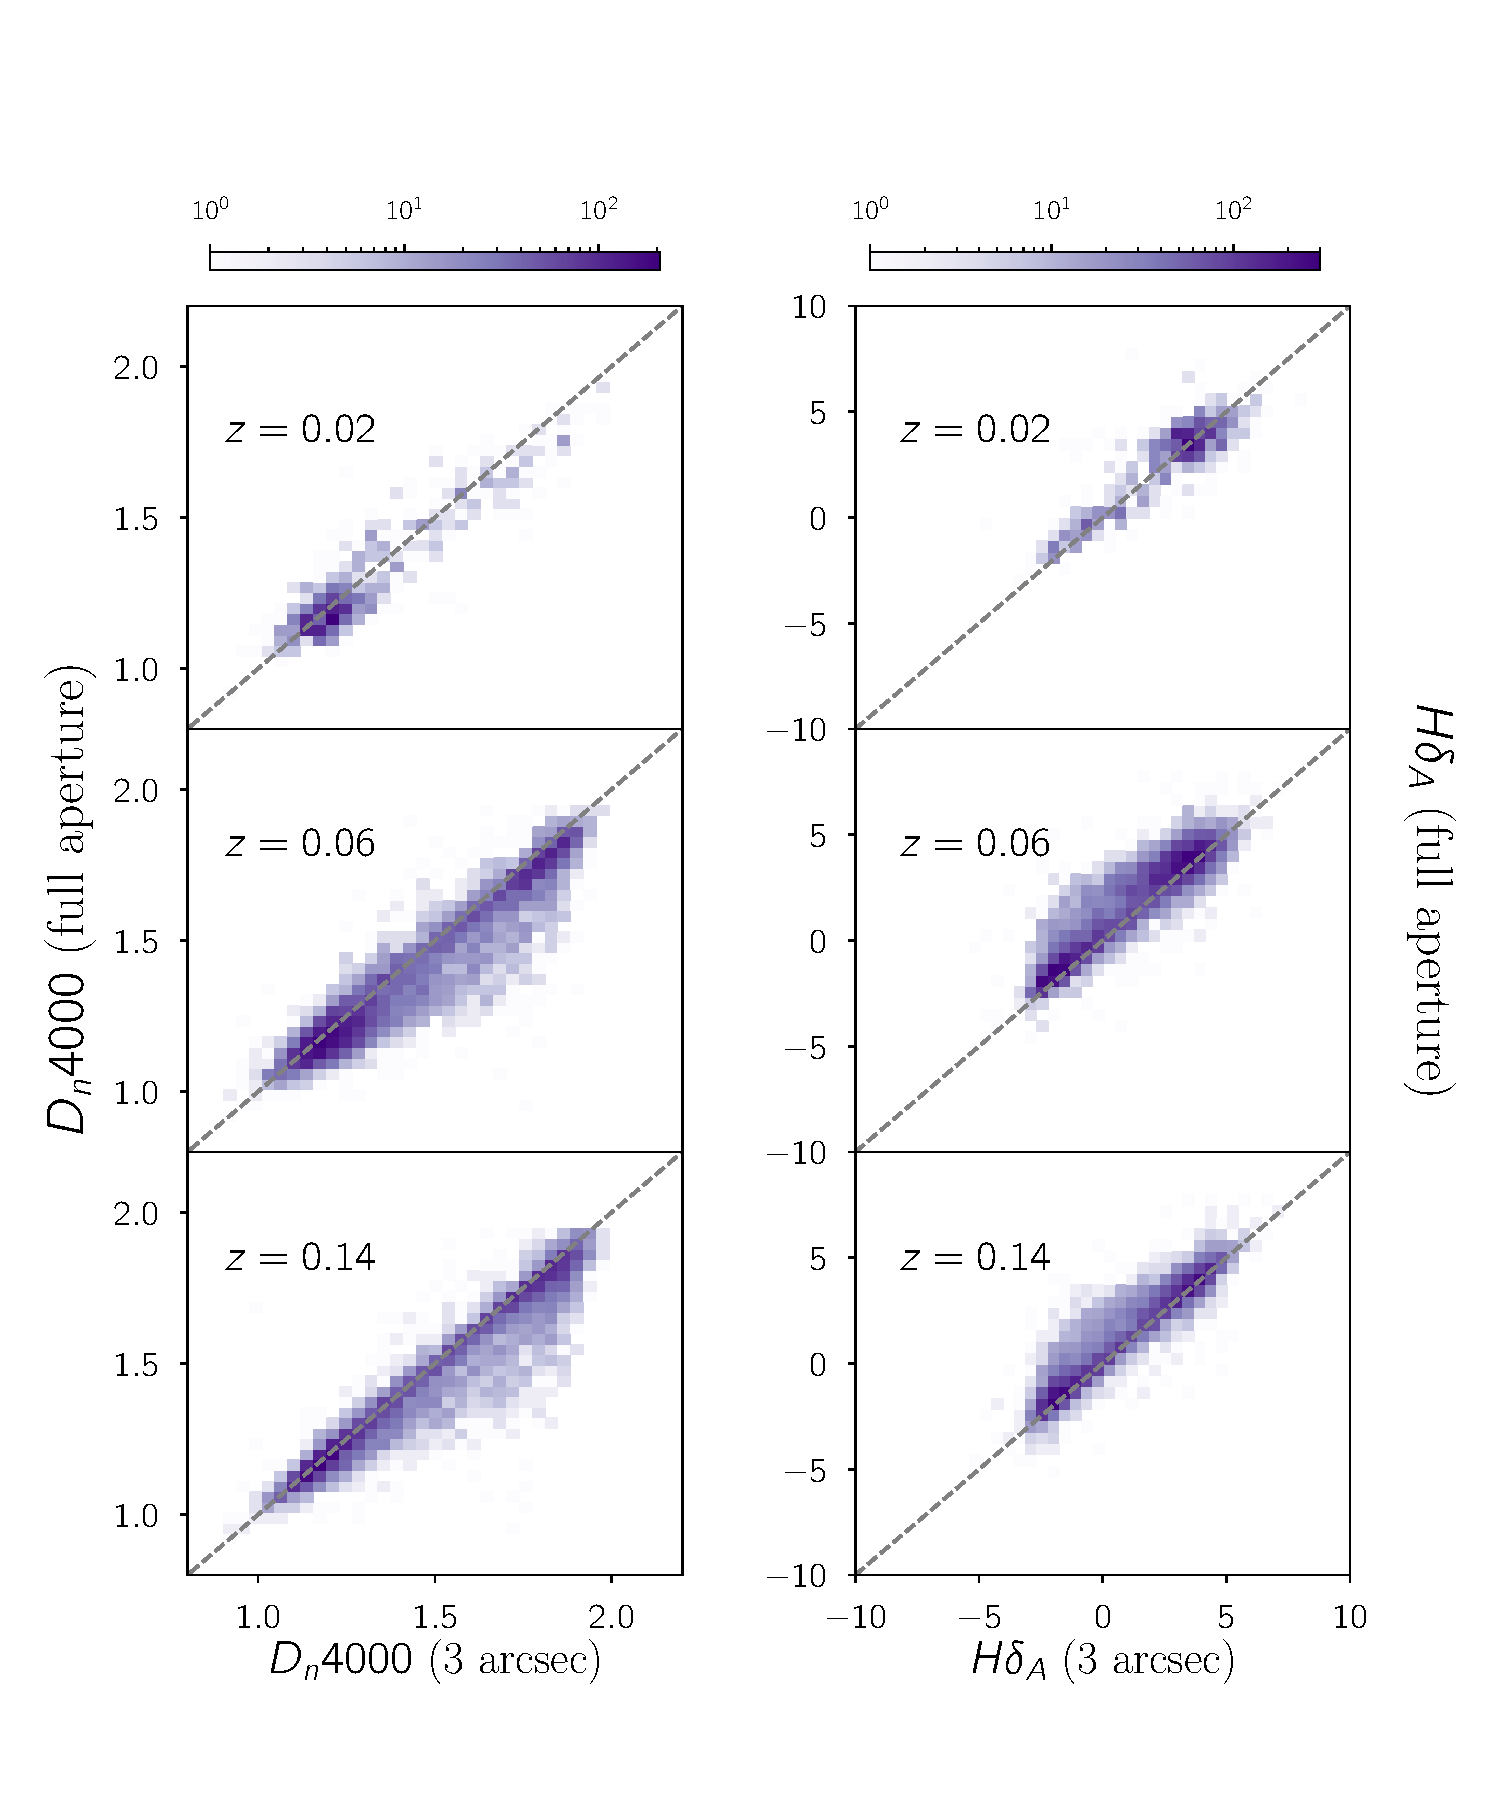
\includegraphics[width=\textwidth]{figures/full_aperture_comparisons.pdf}
\caption[The $D_{n}4000$, $h\delta_{A}$ indices measured at $z = 0.02,0.06,0.14$ with a $3''$ aperture compared to the full aperture measurement]
{ The $D_{n}4000$, $h\delta_{A}$ indices measured at $z = 0.02,0.06,0.14$ with a $3''$ aperture compared to the full aperture measurement
\label{fig:redshift_comparison}}
\end{figure}


\subsection{$H\delta_{\rm A}$, $D_{\rm n}4000$ Measurements within Apertures}
To get the $H\delta_{\rm A}$ and $D_{\rm n}4000$ index measurements for any aperture, we first redshift-correct the spectra obtained from all the spaxels within the aperture to rest-frame. As both the equivalent width of the Balmer $H\delta$ line as well as the $D_{n}4000$ break rely on the continuum as well as a ratio of fluxes in the case of the latter, we add up the spectra of the spaxels that fall within any aperture before estimating either. We then follow the procedure described in Section $2.2$ to calculate the indices. (In a footnote: the code for this is publicly available at --provide github link--.)

\section{Results}
\subsection{Comparison to Full Aperture Measurements}
To investigate how the full aperture measurements compare to the 3'' measurements, we choose 3 different redshift bins $z = 0.02,0.06$ and $0.14$ and observe how offset the $H\delta_{\rm A}$ and $D_{\rm n}4000$ measures are. For each redshift, I pick the galaxies whose redshift are below that redshift and ``shift" them to the cutoff redshift as described in Section \ref{sec:chap2methods} and compare the full aperture measurements to the 3'' measurements made at that redshift. The results of this are shown in Fig. \ref{fig:redshift_comparison}, where the full aperture measurements are plotted against the 3'' measurements at the respective redshifts with the colorbars indicating the number of galaxies in each bin. We note that the total number of galaxies in each redshift bin is 561 for $z = 0.02$, 5016 for $z = 0.06$ and 6402 for $z = 0.14$.\\

\begin{figure}
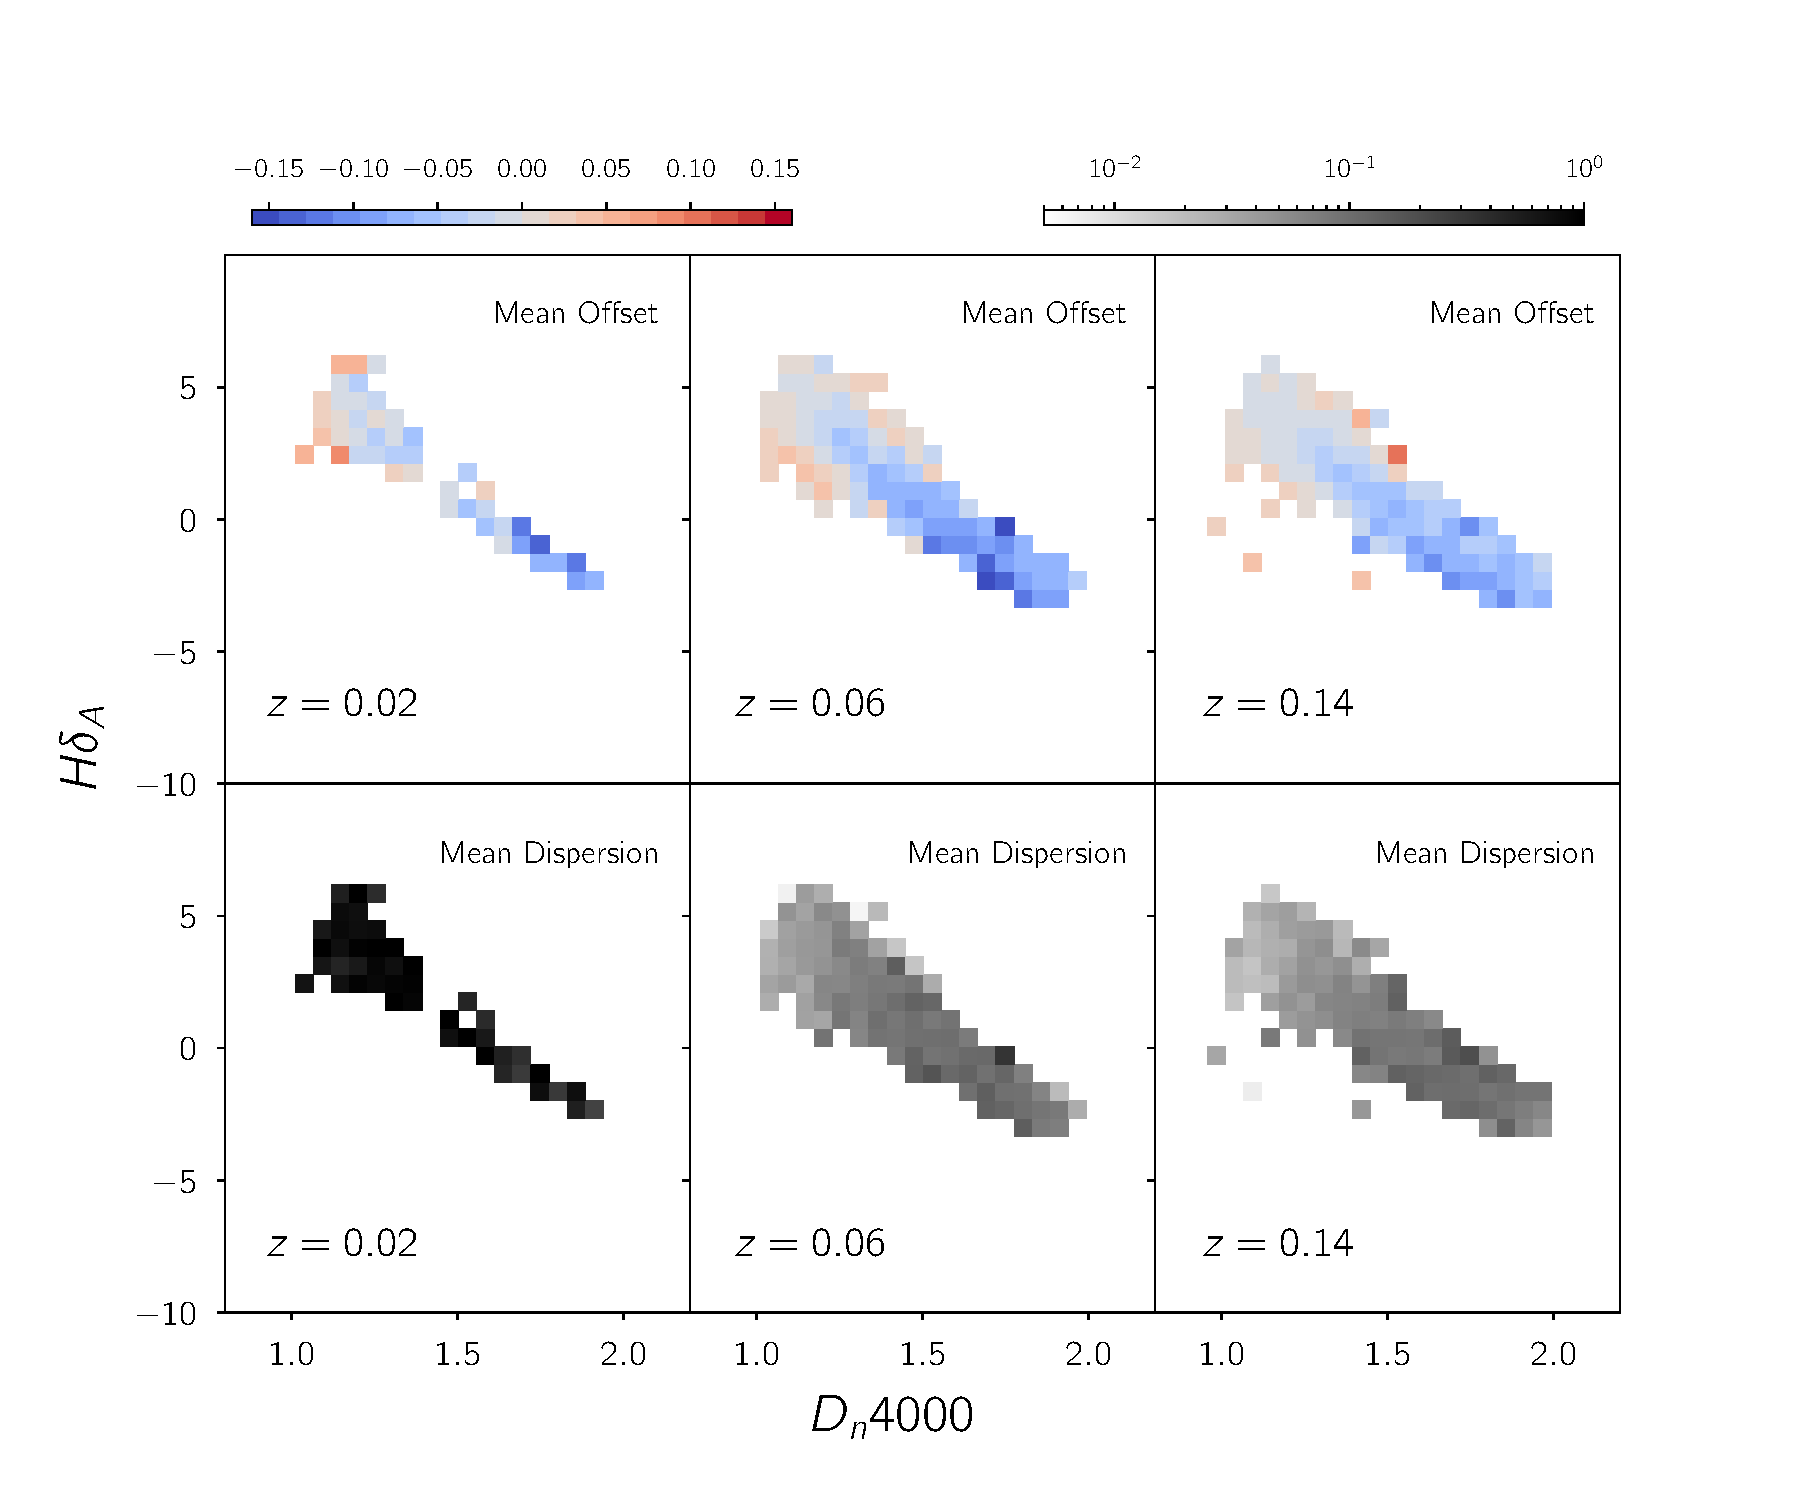
\includegraphics[width=\textwidth]{figures/dn4000_full_aperture_comparisons.pdf}
\caption[The mean offset and dispersion in the $D_{n}4000$ index measured at $z = 0.02,0.06$ and $0.14$ with a $3''$ aperture from the full aperture measurement]{ The mean offset and dispersion in the $D_{n}4000$ index measured at $z = 0.02,0.06$ and $0.14$ with a $3''$ aperture from the full aperture measurement
\label{fig:offset_d4000}}
\end{figure}

From Fig. \ref{fig:redshift_comparison}, we can infer the following. For most of the galaxies the offset is pretty minimal as it as they fall pretty close to the $x=y$ line. We find that the scatter is the most at $z = 0.06$ and tends towards higher $D_{\rm n}4000$ and lower $H\delta_{\rm A}$ values relative to the full aperture measurements. This can be interpreted as the effect of the apertures beginning to cover the galaxy disks which have lower star formation activity than the bulge for galaxies with strong bulges. The scatter lessens as we approach $z = 0.14$, close to the survey limit, where for most of the galaxies, all of the light gets accounted for by the 3''aperture at this point.\\

\begin{figure}
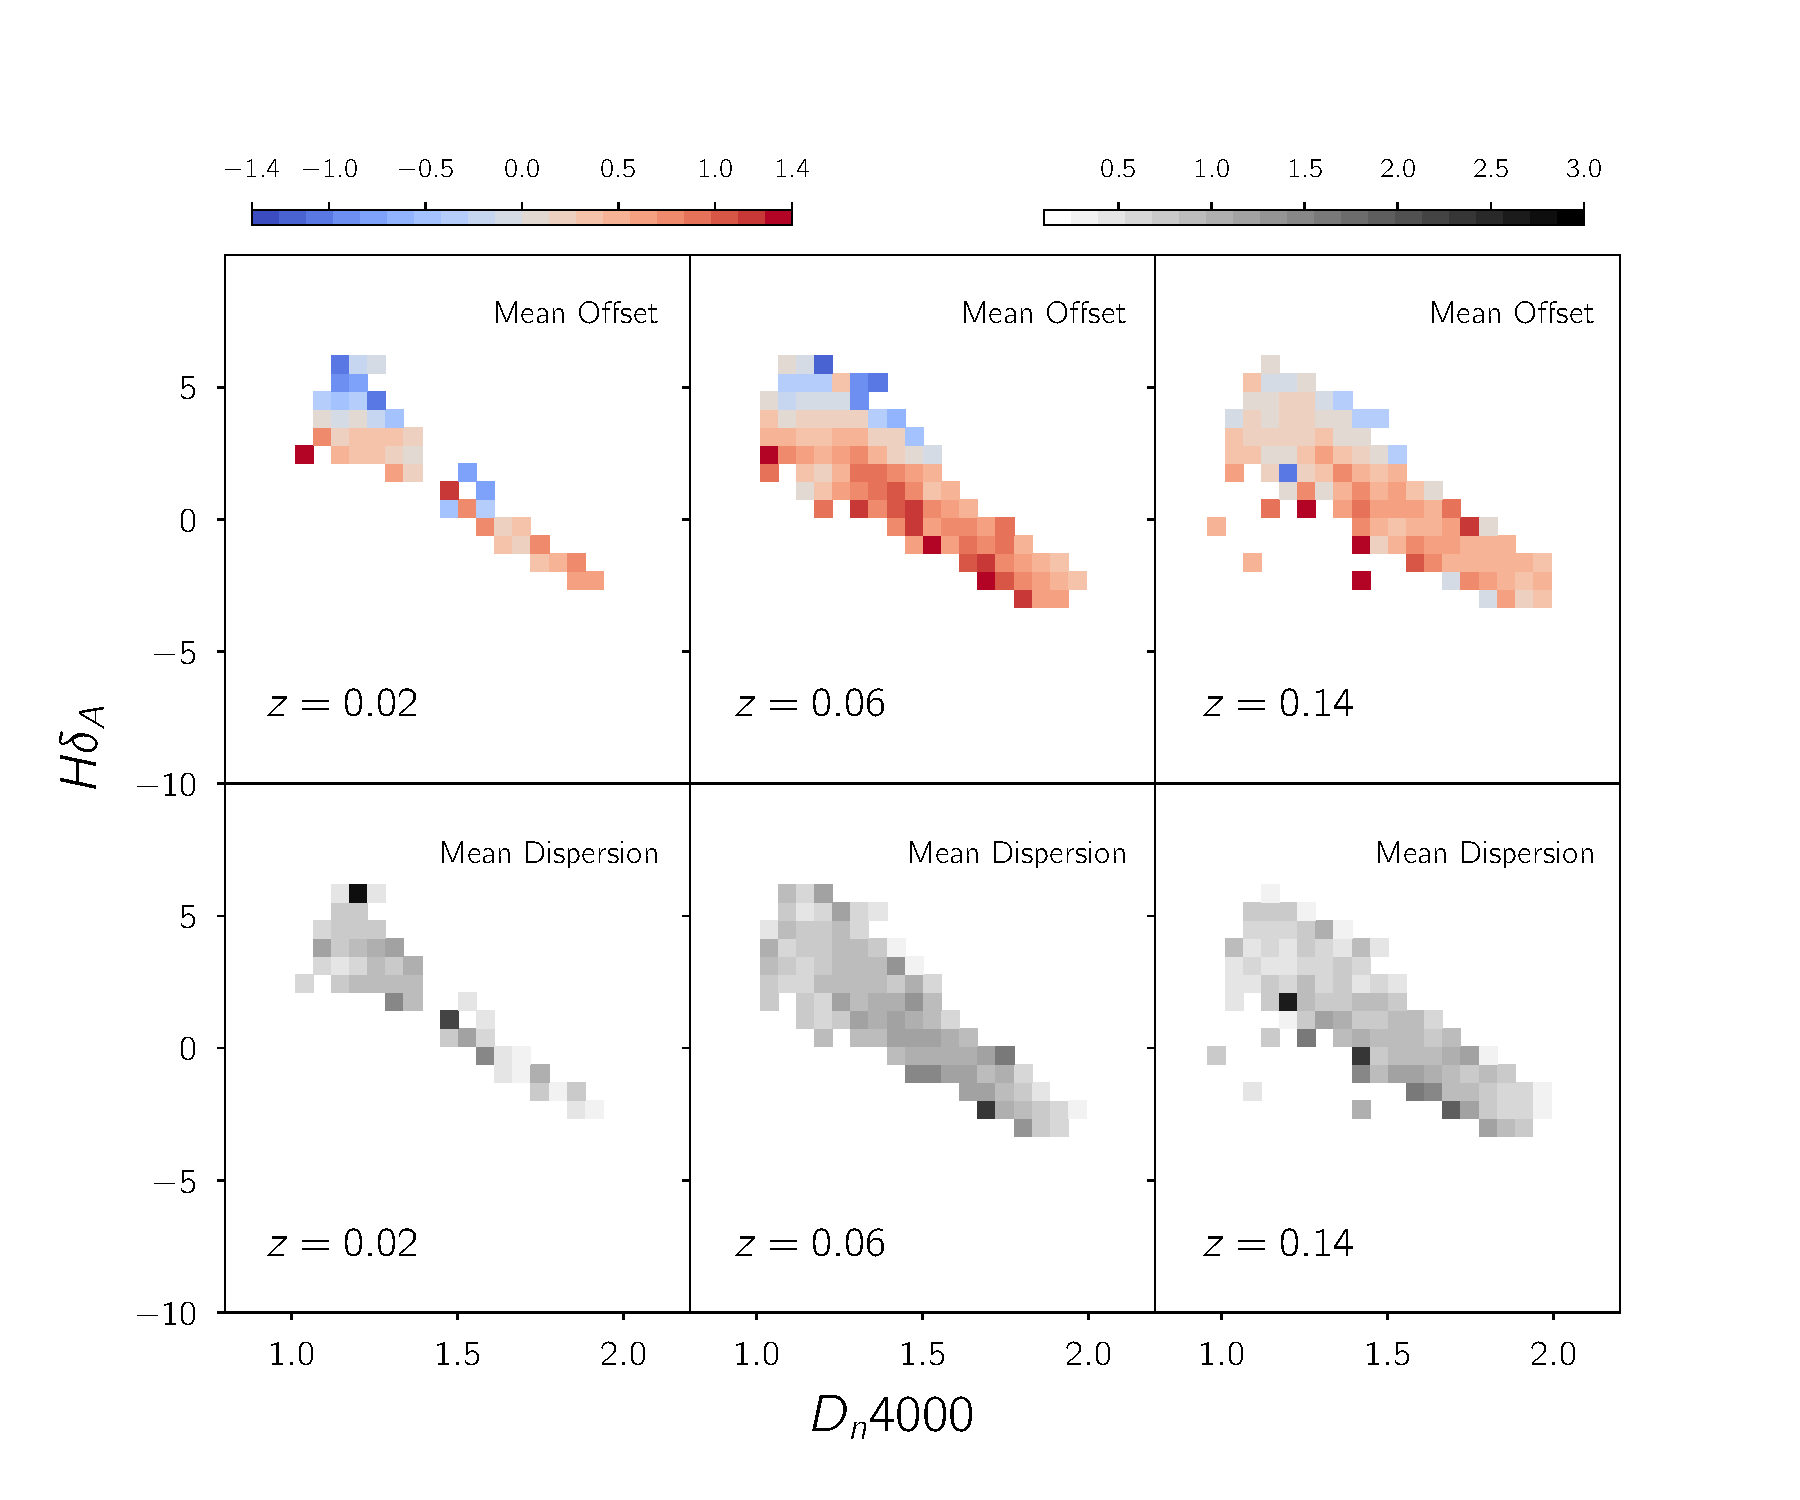
\includegraphics[width=\textwidth]{figures/hdelta_full_aperture_comparisons.pdf}
\caption[The mean offset and dispersion in the $h\delta_{A}$ index measured at $z = 0.02,0.06$ and $0.14$ with a $3''$ aperture from the full aperture measurement ]{ The mean offset and dispersion in the $h\delta_{A}$ index measured at $z = 0.02,0.06$ and $0.14$ with a $3''$ aperture from the full aperture measurement 
\label{fig:offset_hdelta}}
\end{figure}

MRB Says: At all redshifts, we can see that there is a systematic tendency for galaxies to appear older through the fiber aperture than through the full aperture, and therefore to appear to have a higher M/L than they actually do. This would particularly affect the intermediate age galaxies (i.e. those with $D_{\rm n}4000$ in the green valley).\\


\subsection{Offsets in the $H\delta_{\rm A}$-$D_{\rm n}4000$ plane}

\begin{figure}
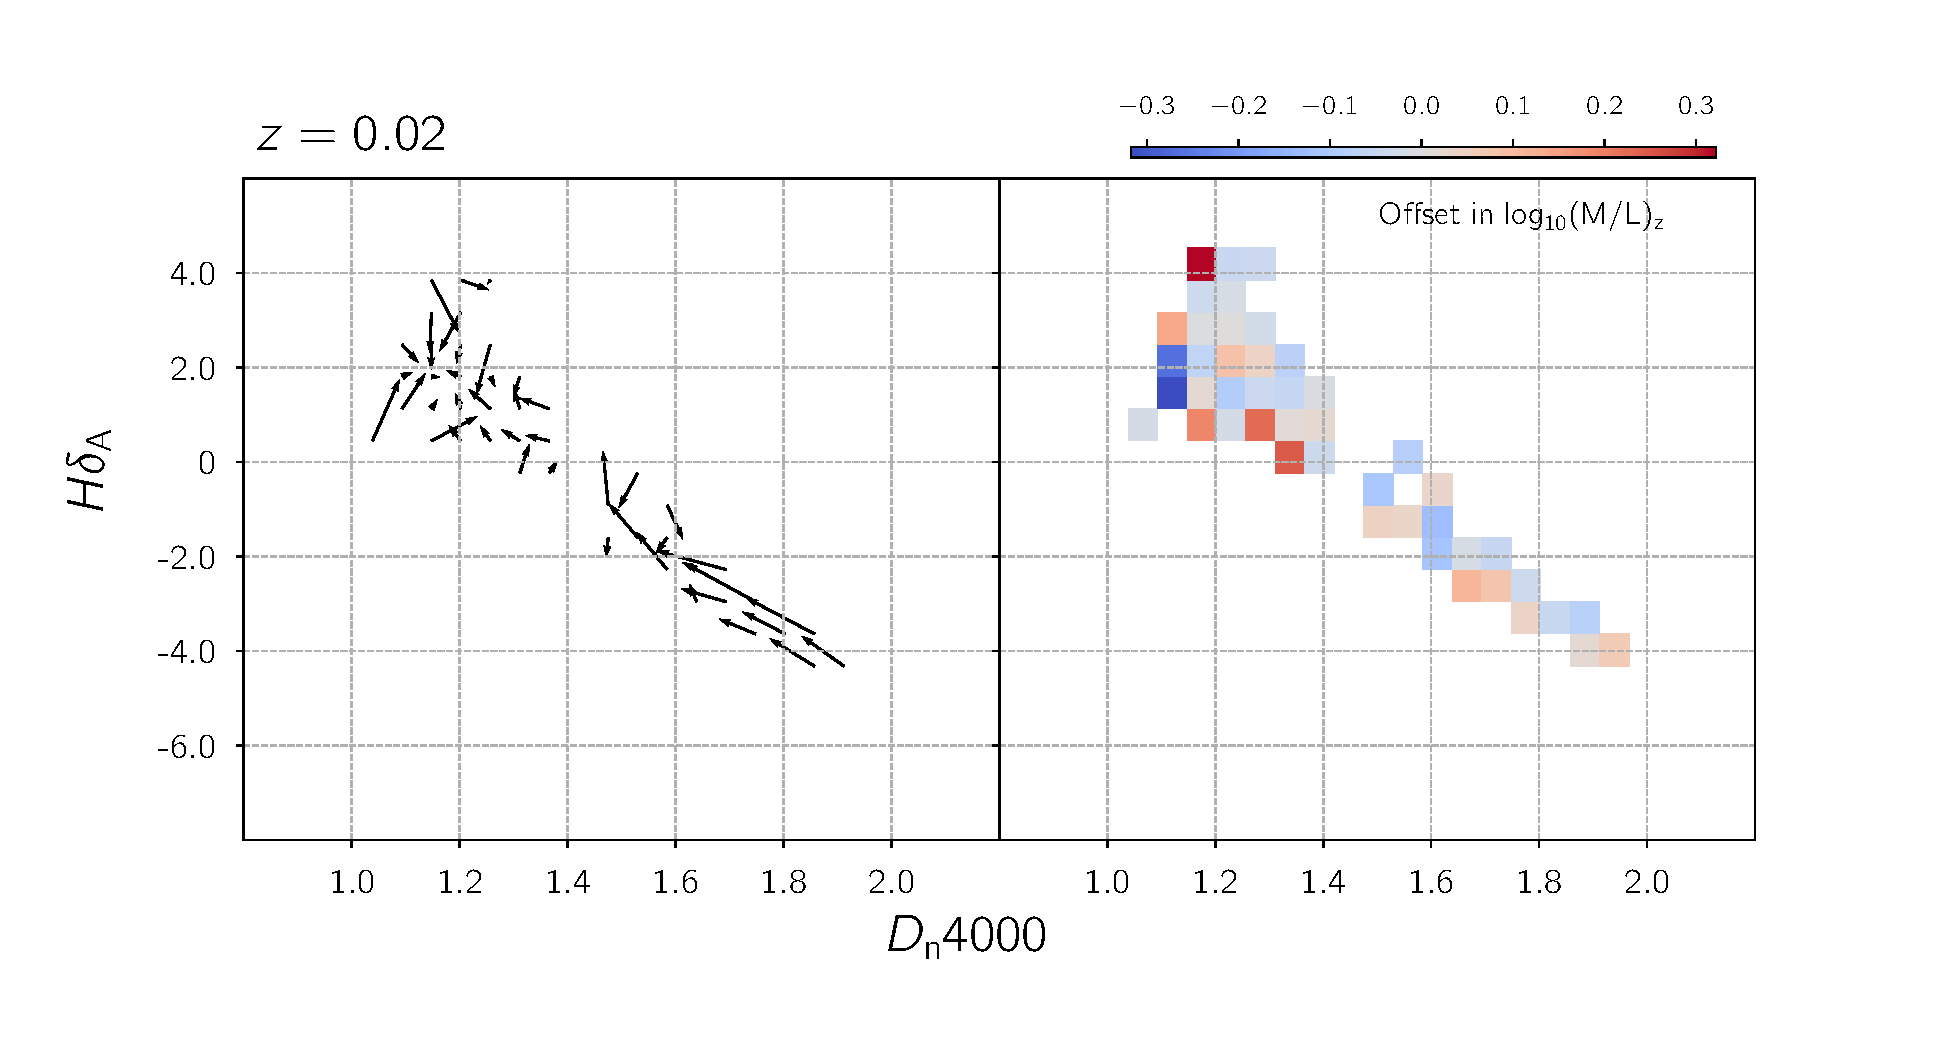
\includegraphics[width=\textwidth]{figures/mlz_offset_a.pdf}
\caption[  \emph{Left:} The combined mean offset in $D_{\rm n}4000$-$h\delta_{\rm A}$ at $z=0.02$ from the full aperture measurements represented as a vector whose projections on the axes are the actual offsets in either direction. \emph{Right:} The offsets transformed to the z-band mass-to-light ratios using the grid in Figure \ref{fig:kauff_grid}. ]{ \emph{Left:} The combined mean offset in $D_{\rm n}4000$-$h\delta_{\rm A}$ at $z=0.02$ from the full aperture measurements represented as a vector whose projections on the axes are the actual offsets in either direction. \emph{Right:} The offsets transformed to the z-band mass-to-light ratios using the grid in Figure \ref{fig:kauff_grid}.
\label{fig:offset_quiver1}}
\end{figure}


\begin{figure}
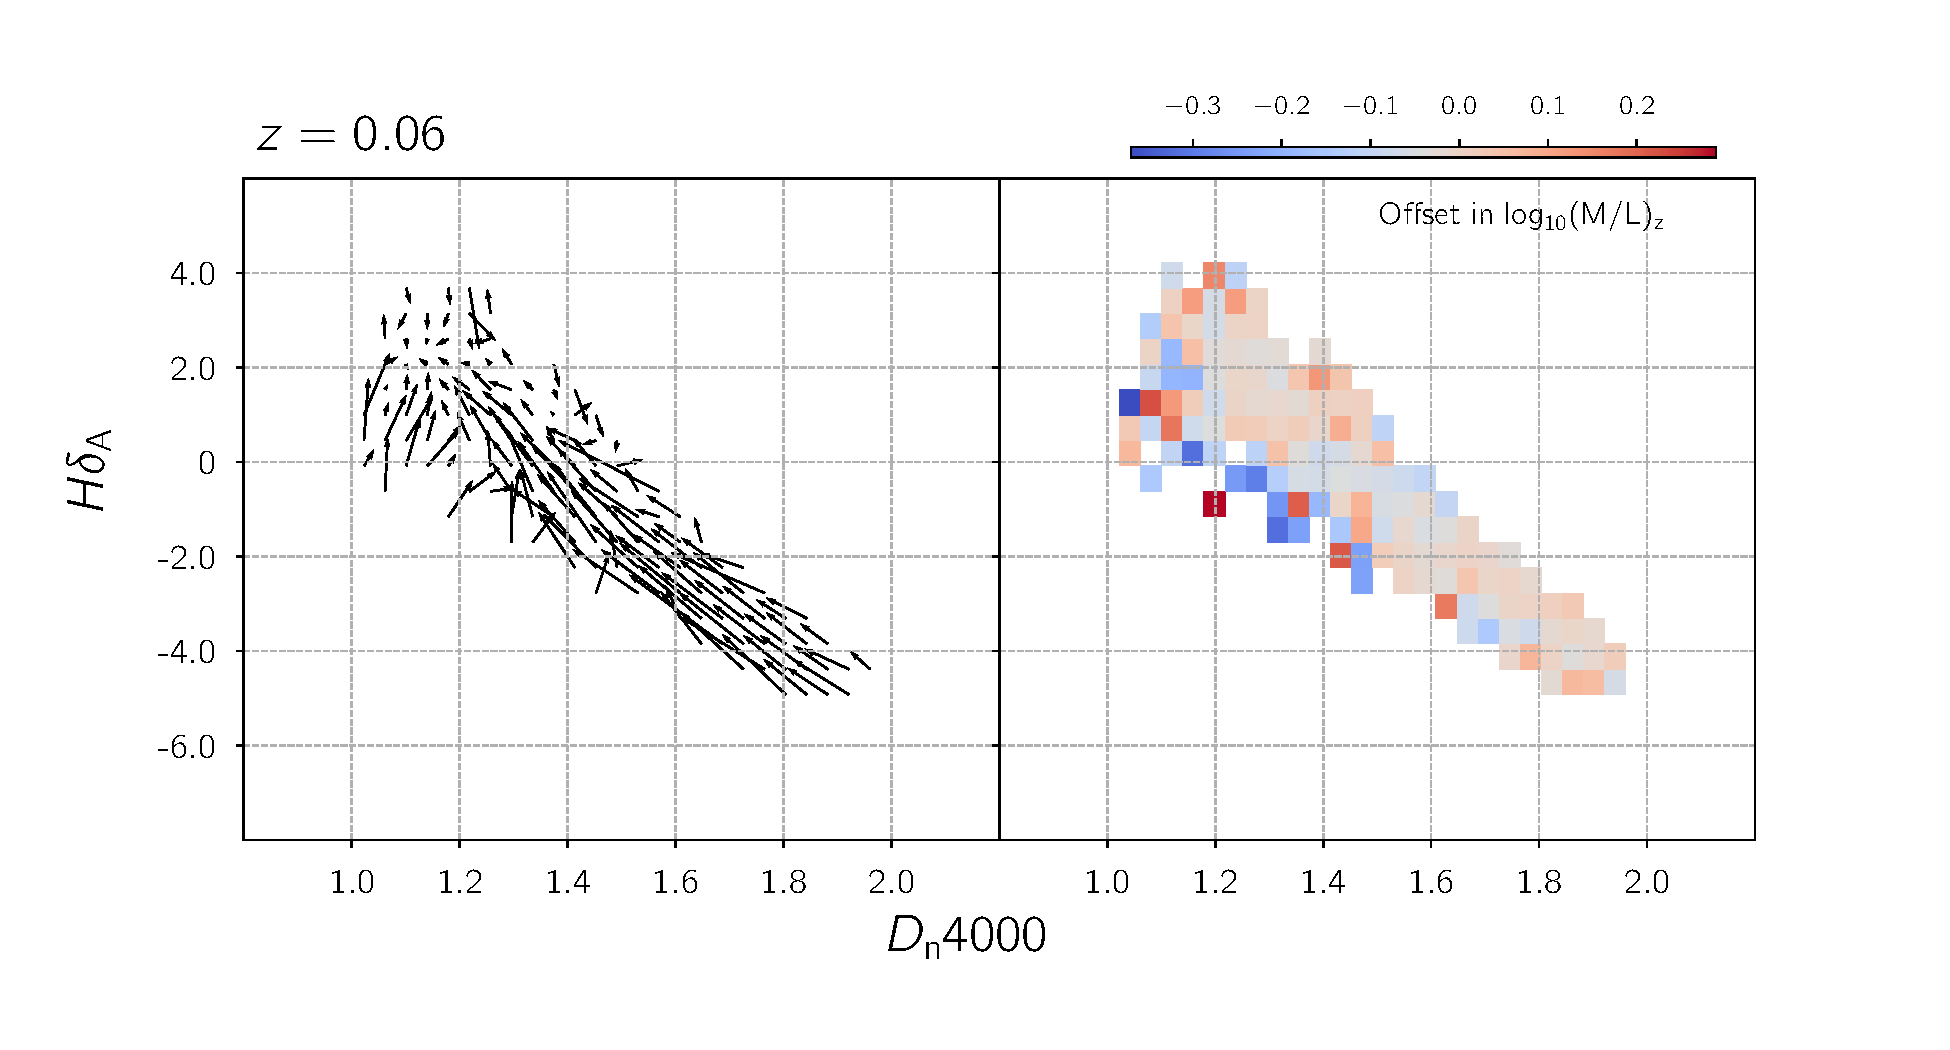
\includegraphics[width=\textwidth]{figures/mlz_offset_b.pdf}
\caption[  \emph{Left:} The combined mean offset in $D_{\rm n}4000$-$h\delta_{\rm A}$ at $z=0.02$ from the full aperture measurements represented as a vector whose projections on the axes are the actual offsets in either direction. \emph{Right:} The offsets transformed to the z-band mass-to-light ratios using the grid in Figure \ref{fig:kauff_grid}. ]{ \emph{Left:} The combined mean offset in $D_{\rm n}4000$-$h\delta_{\rm A}$ at $z=0.06$ from the full aperture measurements represented as a vector whose projections on the axes are the actual offsets in either direction. \emph{Right:} The offsets transformed to the z-band mass-to-light ratios using the grid in Figure \ref{fig:kauff_grid}.
\label{fig:offset_quiver2}}
\end{figure}

\begin{figure}
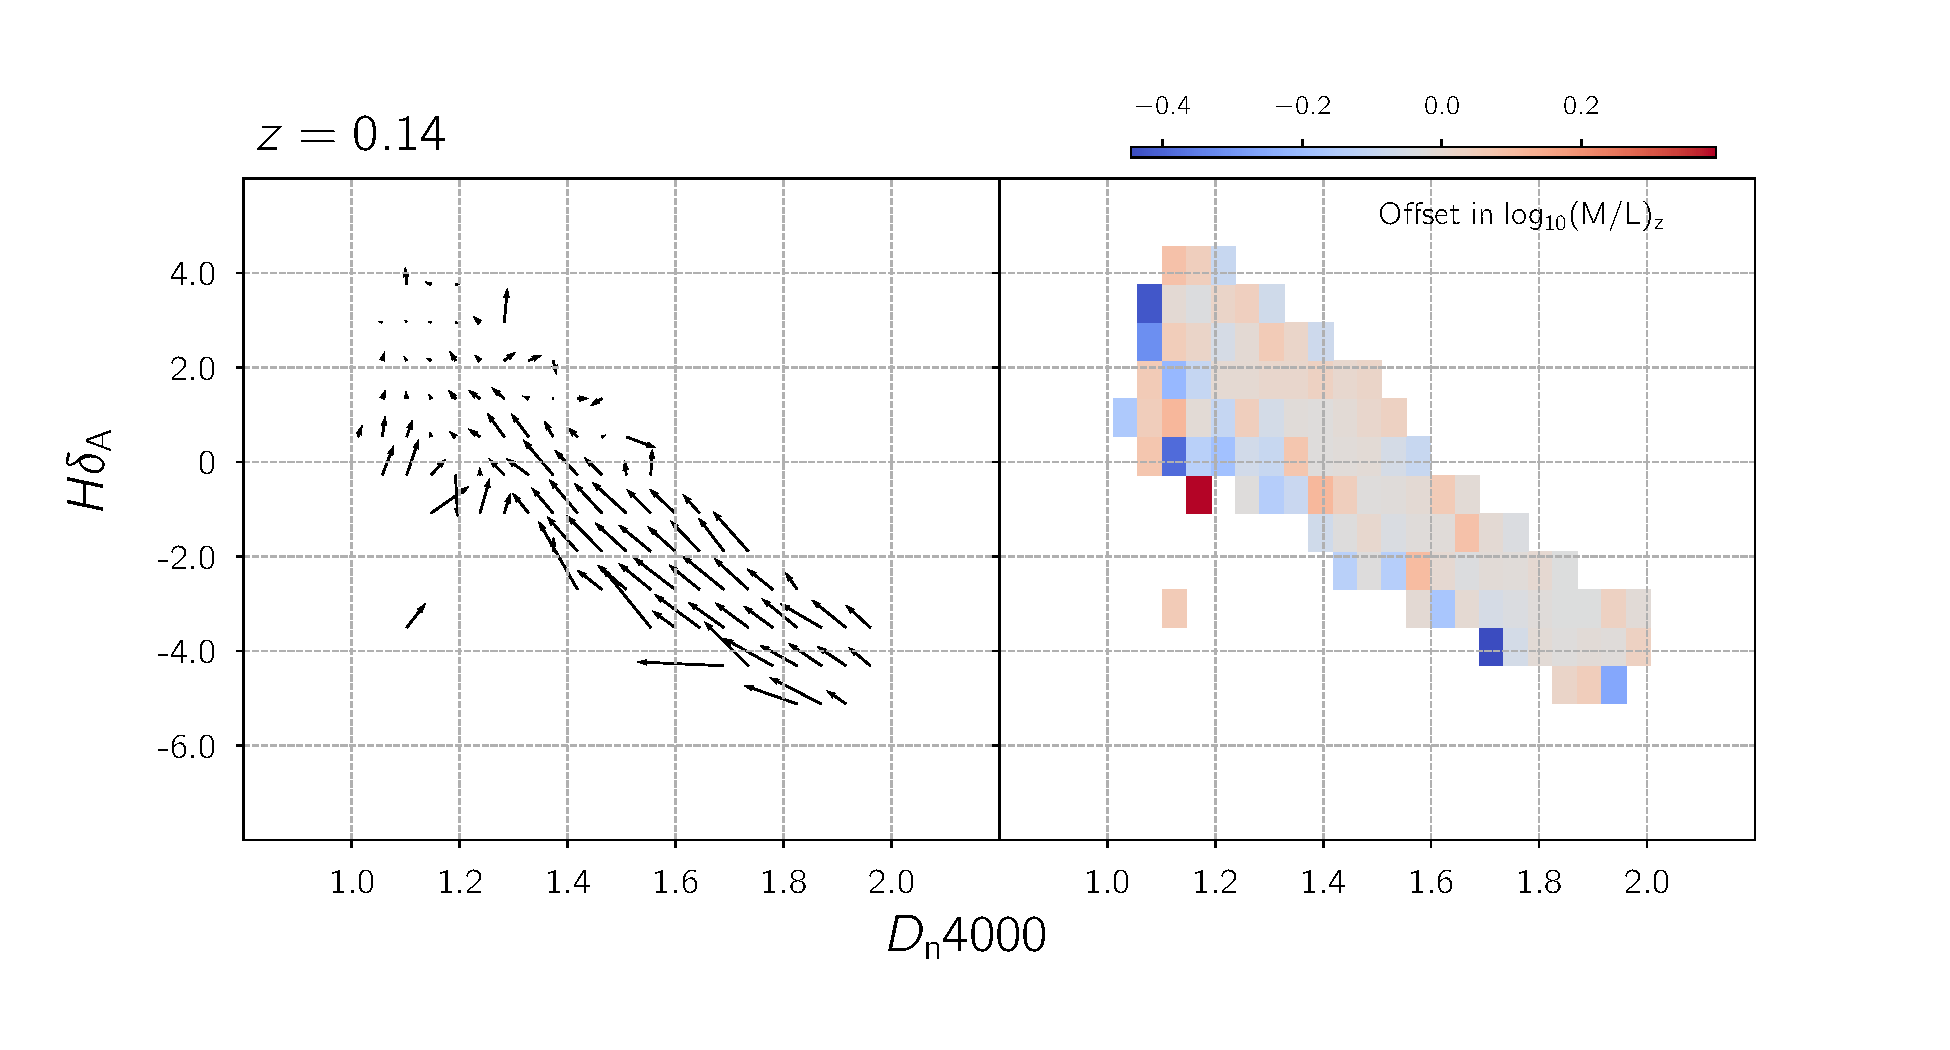
\includegraphics[width=\textwidth]{figures/mlz_offset_c.pdf}
\caption[ \emph{Left:} The combined mean offset in $D_{\rm n}4000$-$h\delta_{\rm A}$ at $z=0.14$ from the full aperture measurements represented as a vector whose projections on the axes are the actual offsets in either direction. \emph{Right:} The offsets transformed to the z-band mass-to-light ratios using the grid in Figure \ref{fig:kauff_grid}. ]{ \emph{Left:} The combined mean offset in $D_{\rm n}4000$-$h\delta_{\rm A}$ at $z=0.14$ from the full aperture measurements represented as a vector whose projections on the axes are the actual offsets in either direction. \emph{Right:} The offsets transformed to the z-band mass-to-light ratios using the grid in Figure \ref{fig:kauff_grid}.
\label{fig:offset_quiver3}}
\end{figure}

\section{Discussion}

MRB Says: * This mean tendency is *relatively* small. You should calculate from your grids the median offset for cells with D4000 > 1.3 or something like that, and quote that number. You should then look carefully at the Kauffmann figure to translate this to a change in $M/L_z$ --- my guess is that it is around 0.1 dex for z=0.06. Do this for z=0.06 and z=0.14.

 * The scatter about this mean is substantial relative to the mean. Again, calculate the median standard deviation over the cells with D4000 > 1.3 to quantify this. My guess is that it is  comparable to the mean itself. This means for individual galaxies the error can be a lot bigger. Again quote for both those redshifts.

 * The main conclusion is that stellar masses more accurate than 0.1 dex (or whatever you see in the mean offset) arenot possible, and that the scatter in the offset means the precision is degraded as well. This source of error is important
to keep in mind but is probably not fatal for samples at z=0.1
from MPA/JHU --- most results done rely on stellar masses
at that precision. Using this sample at lower redshift may be
much more iffy.







